\section{Vector Autoregressive model}
\label{sec:VAR}
Vector Autoregressive (VAR) models are used in time series research to study the dynamic relationships between interacting variables. Additionally, they serve as forecasting tools. \\
These models extend the single-variable (univariate) Autoregressive model discussed in Chapter 2 to handle multiple time series. The main difference is that VAR models allow for feedback between variables.\\\\
A basic VAR model describes the evolution of $K$ target variables over time. These variables are collected in a vector $\mathbf{y}_t = (y_{1t}, ..., y_{Kt})$ of length $K$. Each VAR model is characterized by its order, which indicates the number of past time periods the model uses. A lag refers to the value of a variable in a previous time period. Generally, a $p$th-order VAR includes lags from the last $p$ time periods and is denoted as "VAR(p)". It can be written as:
\begin{equation}
    \mathbf{y}_t = A_1 \mathbf{y}_{t-1} + A_2 \mathbf{y}_{t-2} + \cdots + A_p \mathbf{y}_{t-p} + \mathbf{\epsilon}_t,
\end{equation}
where:
\begin{itemize}
    \item \(\mathbf{y}_t\) is a \(k \times 1\) vector of variables at time \(t\),
    \item \(A_i\) (for \(i = 1, 2, \ldots, p\)) are \(k \times k\) coefficient matrices,
    \item \(\mathbf{\epsilon}_t\) is a \(k \times 1\) vector of error terms.
\end{itemize}
Assuming \(\mathbf{\epsilon}_t\) is white noise with normal distribution, zero mean and a constant covariance matrix \(\Sigma\), we have:
\begin{equation}
    \mathbf{\epsilon}_t \stackrel{iid} \sim \mathcal{N}(0, \Sigma)
\end{equation}
For which concern our case, we implemented the VAR(1) model, resulting in the following formulation:
\begin{equation}
    \mathbf{y}_t = A \mathbf{y}_{t-1} + \mathbf{\epsilon}_t,
\end{equation}
or, in a more extensive way:
\begin{equation}
    \label{VAR_1}
    \begin{pmatrix}
        y_{1t} \\
        y_{2t}
    \end{pmatrix}
    =
    \begin{pmatrix}
        a_{11} & a_{12} \\
        a_{21} & a_{22}
    \end{pmatrix}
    \begin{pmatrix}
        y_{1, t-1} \\
        y_{2, t-1}
    \end{pmatrix}
    +
    \begin{pmatrix}
        \epsilon_{1t} \\
        \epsilon_{2t}
    \end{pmatrix}
\end{equation}
where:
\begin{itemize}
    \item \(y_{1t}\) is the GDP\_PC1 variable at time t.
    \item \(y_{2t}\) is the CPIAUCSL\_PC1 variable at time t.
\end{itemize}

\section*{VAR(1)}
Given the equation \ref{VAR_1} the likelihood of the VAR model is as follows:
\begin{equation}
    \mathbf{y}_{t}|\mathbf{\mu}_{0}, A, \Sigma, \mathbf{y}_{t-1} \sim \mathcal{N}_2(\mathbf{\mu}_{0} + A \mathbf{y}_{t-1}, \Sigma)
\end{equation}
and we selected the following priors:
\begin{equation}
    \begin{split}
        \mu_{0i} \sim \mathcal{N}(0.0, 10000) \quad i = 1, 2\\
        A_{ij} \sim \mathcal{U}(-1, 1) \quad i,j = 1, 2 \\
        \Omega = \Sigma^{-1} \sim Wishart(R, 3)
    \end{split}
\end{equation}
where:
\begin{equation}
    R = 
    \begin{pmatrix}
        1 & 0.5 \\
        0.5 & 1
    \end{pmatrix}
\end{equation}
choosing them to be uninformative ones. \\
We produced the traceplots and autocorrelation plots to verify the validity of our assumptions and we obtained the following posteriors for the parameters: \\
\begin{figure}[h]
    \centering
    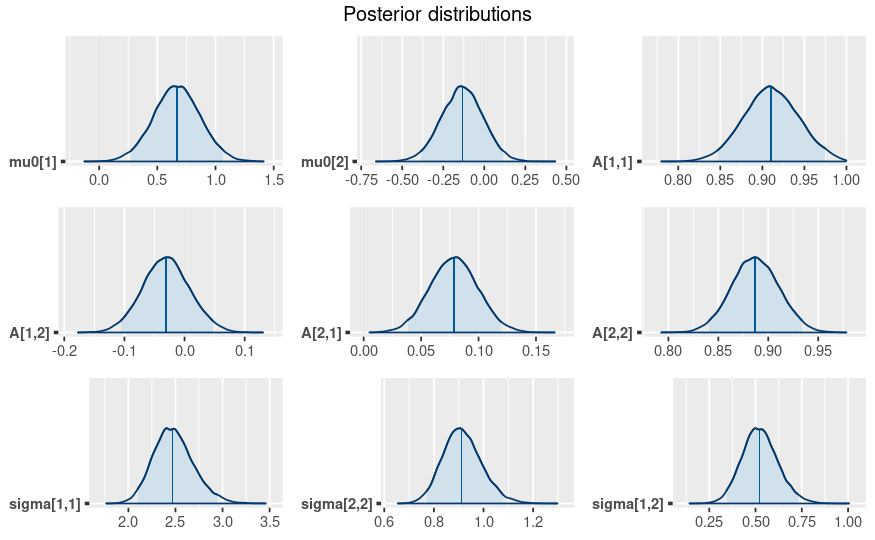
\includegraphics[width=\textwidth]{images/6-VAR/posteriors.png}
    \caption{The image displays the posterior distributions of the parameters for the VAR(1) model.}
    \label{fig:VAR_posteriors}
\end{figure} \\
Finally we plotted the in-sample and out-of-sample predictions with credible intervals and we compared it with the true data: \\   
\begin{figure}[h]
    \centering
    \begin{minipage}[t]{0.7\textwidth}
        \centering
        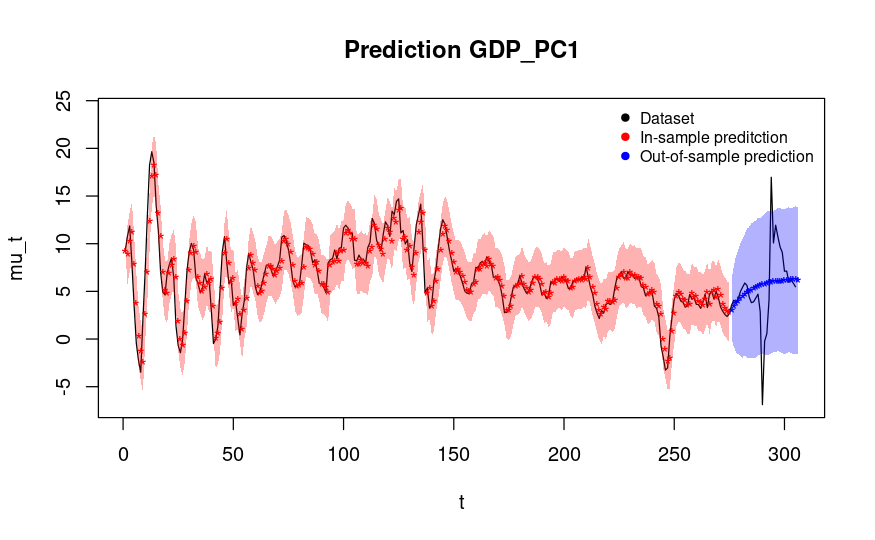
\includegraphics[width=\textwidth]{images/6-VAR/gdp_prediction.png}
        \label{fig:VAR_first}
    \end{minipage}
    \begin{minipage}[t]{0.7\textwidth}
        \centering
        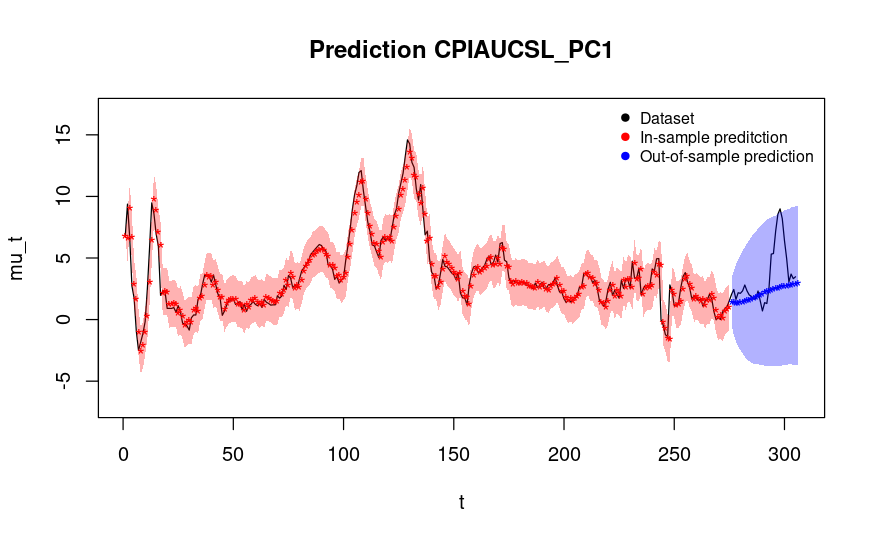
\includegraphics[width=\textwidth]{images/6-VAR/infl_prediction.png}
        \label{fig:VAR_second}
    \end{minipage}
    \caption{VAR(1): In-sample and out-of-sample predictions}
    \label{fig:VAR_combined}
\end{figure}
In the Appendix it is possible to find a comparison between our model and the VAR function (using a frequentistic approach) to verify the model's correctness.